% Hopefully this will be the final version of Problem statement.
\section{Problem Statement}

Cloud providers spend huge amount of money on data centers because a typical data center consumes as much energy as 25,000 households \cite{Dayarathna:2016ua}. Thus, reducing the energy consumption becomes the major concern of Cloud providers. 
In addition, data centers and computation powers are the pillars of modern Cloud computing industry, software industry and etc. Reducing the cost of data centers will lead to a reduction of cost of softwares which consequently be beneficial to most people who access the Internet on a daily basis.
Among several components that consume energy such as cooling system, physical machines (PMs) (e.g servers), and network devices, PMs accounts for 40\% and have a huge improvement space, since they always run in a low utilization as observed by Barroso and Shen \cite{Barroso:2007jt,Shen:2015hm} - from 10\% to 50\% of required resources on average. 

In order to improve the resource utilization as well as reduce energy consumption, one way is cloud resource management \cite{Manvi:2014hm}. Cloud resource management allocates resources to cloud users' applications, handles the workload fluctuations, and attempts to use as fewer number of PMs as possible to save energy. Before virtualization technology \cite{Uhlig:2005do}  was widely used, traditional data center assigns a PM for each application. Later on, PMs' utilization are largely improved by utilizing VMs to deploy applications. However, as a new trend of Service Oriented Architecture \cite{Sprott:2004wt} appears in software industry; It separates a large centralized application into multiple distributed components (e.g web services). As most of web services only require a small amount of resources,  using a VM for a web service would cause resource wastage inside the VM, consequently decreasing the utilization of PMs. Therefore, a new virtualization technology: containers \cite{Felter:2015ki, Soltesz:2007cu} and a new service model: Container as a Service (CaaS) \cite{Piraghaj:2015uf} have been proposed to provide a finer granularity level of resource management. Container is an operating system (OS) level of virtualization which means multiple containers  run on the same VM and share the OS. CaaS uses containers as the fundamental resource management units.  That is, instead of deploying applications on VMs, applications are now deployed in containers which are running on top of VMs. This model lets us minimize the waste of resources as well as energy consumption \cite{Esposito:2016br}. Although this new technology gives an opportunity for better resource utilization, it also poses challenges to server consolidation. 
% is a mixture of traditional IaaS (Infrastructure as a Service) \cite{Mell:2011jj} and PaaS (Platform as a Service); it 


\begin{figure}
	\centering
	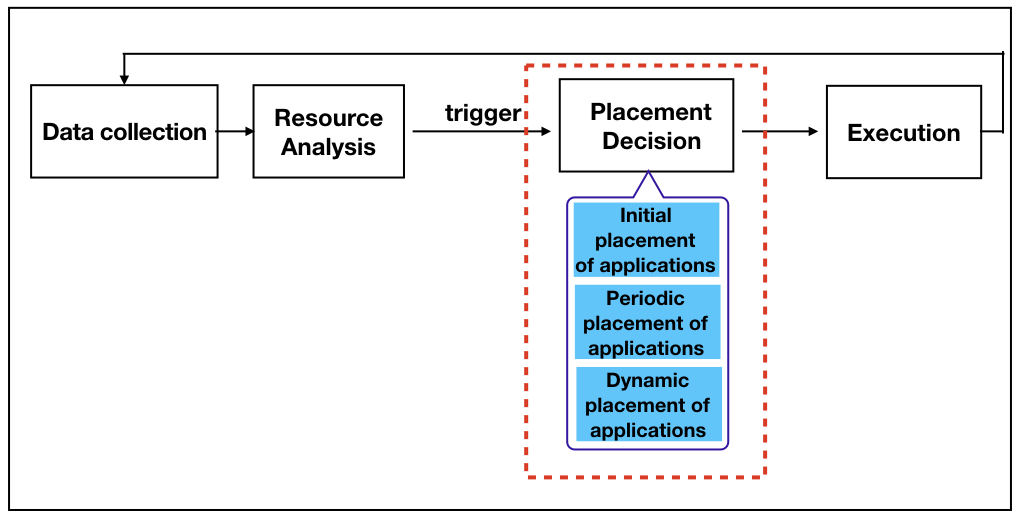
\includegraphics[width=0.7\textwidth]{pics/workflow_management.png}
	\caption{A workflow of resource management \cite{Mishra:2012kx}}
	\label{fig:workflow}
\end{figure}

Server consolidation \cite{Varasteh:2015fu} is the core strategy in improving the utilization as well as decreasing the overall energy consumption throughout the Cloud resource management processes as shown in Figure \ref{fig:workflow}. Server consumption is essentially an optimization task where it adjusts applications' locations in PMs so that a minimum number of PMs is used. For a certain number of applications, the fewer number of PMs is used, the less energy is consumed. 

Three management processes: application initial placement \cite{Jennings:2015ht}, periodic optimization \cite{Mishra:2012kx}, overloading and under-loading adjustments \cite{Mishra:2012kx} have distinct characteristics, hence, the server consolidation techniques applied on them can be roughly classified into two categories: static \cite{Xiao:2015ik} and dynamic \cite{Beloglazov:2012bw}.
Static approaches use estimated resource utilization of applications (e.g average resource utilization of historical data) as the input to combine applications to a minimum number of PMs \cite{Mishra:2012kx}. Static consolidation normally involves large number of applications and PMs, therefore, the optimization is quite time-consuming and often conducted in an off-line and a proactive (Cloud providers initiate) fashion. Periodic optimization belongs to this category. It takes a number of existing applications and re-allocate them into a number of PMs. 

Static server consolidation are detailed explained in terms of VM-based and container-based Cloud. In a traditional VM-based Cloud, server consolidation can be described as, given a number of  PMs which can be represented as resources (e.g CPU cores and RAM etc); a number of requests for fixed configurations of VMs (assume applications have been deployed in VMs), the configuration can also be represented as aforementioned resources; The objective is to allocate these requested VMs into a minimum number of PMs. The decision variable is the location of each requested VM. The basic constraint is that the aggregative resources  of hosted VMs cannot exceed the PM's resource capacity. 

In contrast, in a container-based Cloud, instead of allocating requested VMs in PMs, a set of containers (assume applications have been deployed into containers) represented as resources is first allocated to a number of fixed type VMs, we define it as the lower level of allocation. Then, these VMs are allocated to PMs, this is the upper level of allocation. The decision variables are the allocation of containers to VMs (lower level) and the allocation of VMs  to PMs (upper level). For the lower level of allocation, the objective is to maximize the utilization of resources (e.g a balanced utilization among several resources), while the upper level objective is to minimize the number of PMs. The constraint is the demand of containers not to exceed the VM's capacity and the demand of hosted VMs not to exceed the PM's resource capacity. An additional constraint is that each container has its OS requirement which makes them cannot be simply packed into homogeneous VMs. 

We consider application initial placement and periodic optimization as static consolidation. The main differences between these two processes are, initial placement is a single objective task, where a batch of applications is placed to PMs and the objective is the minimize the overall energy consumption. We consider the placement according to their required resources, therefore, the demand is considered static. In contrast, periodic consolidation takes existing applications' placement, re-placing them to PMs according to the nature of their workloads (e.g static, periodic or continuously changing). It is a multi-objective task which considers minimizing the migration of applications and minimizing the overall energy consumption. That is, the migration is an expensive operation. 


Dynamic approaches take one application each time, allocate it into one of the PMs \cite{Xiao:2015ik}. As a dynamic problem often requires fast reaction such as overloading and underloading problems \cite{Beloglazov:2013ht},
% - A PM is overloaded if its load exceeds its capacity in at least one resource. One or more VMs inside must be migrated to other PMs.  A PM is underloaded if all of resources are below a predefined threshold. All VMs inside the PM will be migrated to other PMs. - 
the dynamic consolidation is conducted in an online fashion. Another difficult is that, similar as periodic consolidation, different types of workload also need to be considered in the dynamic task, in order to match the migrated task with the existing applications in PMs. In VM-based Cloud, the dynamic problem can be described as given a set of VMs and PMs, allocating these VMs to PMs iteratively so that the final solution reaches a near-optimal state.
The key point is that the migration of VM can be conducted immediately after its position is decided. Hence, essentially, the problem can be simplified to allocating one VM to PMs. The difficulty is that the iterative process is hard to reach a global optimal because it normally follows a greedy-based approach such as First Fit. In container-based Cloud,  the problem is even complicated, if no VM can accommodate a container, a new VM must be created, which incurs a second level of deployment.

Application initial placement can be seen as either static: allocate a batch of new applications, or dynamic: allocate a new application each time. In this thesis, we will consider it in both ways.

Traditional VM-based server consolidation are modeled as bin-packing problems \cite{Mann:2015ua}. This is because VMs and PMs are naturally modeled as items and bins. Furthermore, server consolidation and bin-packing have the same optimization objective: minimize the number of bins/PMs. The complexity of bin-packing problem is NP-hard which means it is extreme time-consuming to find its optimal solution when the number of decision variables is large. Container-based server consolidation can be categorized as a bilevel optimization problem \cite{Colson:2007bu}. Bilevel optimization problems contain two level of optimization task: the outer optimization task is referred as the upper level task and the inner task is referred as the lower level task. The hierarchical optimization are typically non-convex and strongly NP-hard \cite{Vicente:1994ie}. In our problem, two levels of optimization are both bin packing problems and they are cooperating.

Currently, most research focus on VM-based server consolidation and these methods cannot be directly applied on container-based consolidation because of the different structure. Only few research focus on container-based server consolidation problem. One of  research is from Piraghaj and et al \cite{Piraghaj:2015uf}. They first propose a VM-resizing technique that defines the types of VM based on analyzing the historical data from Google cluster data. Then, they propose a two-step allocation: first allocate containers to VMs and then allocate VMs to PMs. They propose simple heuristics on each level of allocation, thus, did not consider the interaction between two levels (see detailed discussion in Section \ref{container-based-placement}). In addition, they propose a dynamic consolidation \cite{Piraghaj:2016bw} using a series simple heuristics such as Random Host Selection Algorithm or First Fit Host Selection. 


Their resource allocation system completely relies on dynamic consolidation without using static methods. Although their system can execute allocation fast, the energy efficiency cannot be guaranteed. Another research  \cite{Mann:2016hx} is the earliest study which realizes when deploying applications or containers, the VM size selection and VM placement should be considered together because they are interact with each other. They apply a fixed VM placement algorithm and considering a series of VM selection algorithms such as simple selection \cite{Ganesan:2012eb},  Multiple selection, Maxsize, Consolidation-friendly. The results also proves that the interaction between two placement cannot be ignore.



% The reasons are mainly from two aspects, firstly, they mainly rely on simple bin-packing algorithms to allocate containers to VMs. As Mann's research \cite{Mann:2015ua} showed, server consolidation is a lot harder than bin-packing problem because of the multi-dimensional of resources, heterogeneous PMs, migration cost etc. Therefore, general bin-packing algorithms do not perform well. Secondly, they use a two-step allocation. Because of the interaction of two allocations, separated optimization approach will lead to local optima \cite{Mann:2016hx}. Therefore, these two allocations should be considered simultaneously.



The overall goal of this thesis is to develop new container-based server consolidation approaches to solve three problems: joint allocation of containers  and VMs, periodic global optimization and dynamic consolidation. 
